\documentclass[10pt,a4paper,twocolumn]{article}

\usepackage[margin=1.7cm]{geometry}
\usepackage{amsmath}
\usepackage{graphicx}
\usepackage{booktabs}
\usepackage{tabularx}
\usepackage{algorithm}
\usepackage{algpseudocode}
\usepackage{hyperref}

\title{A Byte-Table Density Classifier for an Unlabelled Sensor Node}
\author{Julian Joseph Amaro}
\date{September 23, 2026}

\begin{document}
\maketitle

\begin{abstract}
This paper proposes the online path of a density-based classifier for a
low-power vibration-monitoring sensor node. DBSCAN discovers non-round
classes from unlabelled training data, a Gaussian KDE builds one probability
map per class, and each map is sampled onto a $16\times16$ grid and stored
as one byte per cell: a 768-byte model that classifies a query with $K=3$
byte reads and no kernel evaluation. On a sealed 206-point test set, the
stored uint8 lookup agrees with the continuous KDE on 100.0\% of decisions,
and correctly returns \textsc{unknown} at the centre of a ring class where
no training data exists.
\end{abstract}

\section{Proposed pipeline}

This paper proposes the online half of a density-based classifier for a
low-power vibration-monitoring sensor node. Offline, a workstation min--max
scales unlabelled two-dimensional feature vectors, discovers classes with
DBSCAN, fits one Gaussian KDE per class, normalises every map to its own
peak, and samples the maps to byte tables. Only the precomputed tables and
scaling bounds ship to the device. At inference, the device performs a fixed
number of byte reads; it neither retains the training set nor evaluates a
kernel.

The stored value is recovered by

\begin{equation}
\tilde{g}_c(\mathbf{x}_{ij}) = \frac{q_{ij}}{255}.
\label{eq:dequant}
\end{equation}

For $K=3$, grid size $G=16$, and one byte per cell, the table footprint is

\begin{align}
\text{flash} &= K \cdot G^2 \cdot b \notag \\
&= 3 \cdot 256 \cdot 1 = 768\ \text{bytes}.
\label{eq:flash}
\end{align}

The device also stores 16 bytes for four float32 scaling bounds. Nearest-cell
lookup costs $K=3$ byte reads per query; bilinear lookup is available when
smoothing near a cell edge justifies $4K=12$ reads. Algorithm~\ref{alg:lookup}
states the proposed online path.

\begin{algorithm}[!bt]
\caption{Table-lookup classification (online path).}
\label{alg:lookup}
\begin{algorithmic}[1]
\Require Raw query $(x,y)$; $G\times G$ byte tables $Q_c$; training bounds
$(x_{min},x_{max})$, $(y_{min},y_{max})$; grid size $G$; reject threshold
$\tau$
\Ensure Predicted class $\hat{c}$, or \textsc{unknown}
\State $\tilde{x} \gets (x-x_{min})/(x_{max}-x_{min})$
\State $\tilde{y} \gets (y-y_{min})/(y_{max}-y_{min})$
\State $\mathrm{col} \gets \lfloor\tilde{x}G\rfloor$, clipped to $[0,G-1]$
\State $\mathrm{row} \gets \lfloor\tilde{y}G\rfloor$, clipped to $[0,G-1]$
\For{each class $c$}
    \State $v_c \gets Q_c[\mathrm{row},\mathrm{col}]/255$
    \Comment{one byte read}
\EndFor
\State $\hat{c} \gets \arg\max_c v_c$
\If{$v_{\hat{c}} < \tau$}
    \State \Return \textsc{unknown}
\EndIf
\State $p_c \gets v_c / \sum_k v_k$ for each class $c$
\State \Return $\hat{c}$ with distribution $p$
\end{algorithmic}
\end{algorithm}

\section{Application}

The proposed device is a battery-powered machine-condition sensor attached to
a pump or fan. It periodically derives two features from vibration windows and
must classify a new operating regime using a small flash budget. Labelled
failure data are scarce because faults are rare and expensive to induce, while
normal operating regimes can have non-convex feature-space shapes caused by
load and mounting variation. The 784-byte deployed model, consisting of 768
bytes of tables plus 16 bytes of scaling bounds, makes a constant-cost local
decision practical where retaining hundreds of examples or evaluating a KDE
would not be.

\section{Method and setup}

The reproducible synthetic dataset uses seed 20250903 and contains 1,030
two-dimensional points: two noisy crescents with 340 and 300 points, a
300-point ring, and 90 uniform background points. A fixed 60/20/20 split
produces 618 training, 206 validation, and 206 test points. Bounds are
computed from training data alone and scale all three sets; this makes both
$\epsilon$ and grid indices interpretable in $[0,1]^2$. The test set is spent
exactly once, after bandwidth, grid, and threshold choices are frozen using
training and validation data alone.

DBSCAN ran only on the training split with $\epsilon=0.06$ and
\texttt{min\_samples}=8. It discovered three clusters of 209, 198, and 178
points and labelled 33 points as noise. Noise was excluded from KDE fitting
because otherwise background scatter would distort every class map. A Gaussian
KDE was fitted per discovered class. Table~\ref{tab:bandwidth} shows that
validation mean log-likelihood selected $h=0.05$. Each peak-normalised map was
sampled on a $16\times16$ grid, quantised to \texttt{uint8}, and classified
with $\tau=0.12$.

\begin{table}[!bt]
\centering
\caption{Validation bandwidth sweep; the highest mean log-likelihood selects $h=0.05$.}
\label{tab:bandwidth}
\begin{tabular}{@{}r r@{}}
\toprule
$h$ & Mean log-likelihood \\
\midrule
0.03 & 1.668 \\
0.04 & 1.775 \\
0.05 & 1.806 \\
0.06 & 1.767 \\
0.08 & 1.632 \\
0.10 & 1.487 \\
0.12 & 1.353 \\
\bottomrule
\end{tabular}
\end{table}

\section{Evidence}

Figure~\ref{fig:clusters} shows that DBSCAN retains both crescents and the
ring while k-means, even given $k=3$, slices the crescents and cannot represent
the ring's hollow centre. The scaling check supports reporting $\epsilon$ only
in the scaled space. Table~\ref{tab:epsilon} shows that no single
$\epsilon$ works in both raw and scaled feature spaces. The additional
$\epsilon=0.03$ test fragmented the scaled training set into 15 clusters and
labelled 82 points as noise; at $\epsilon=0.30$, the scaled set merged into
one cluster with no noise.

\begin{table}[!bt]
\centering
\caption{The same $\epsilon$, applied in raw and scaled feature space on the training set.}
\label{tab:epsilon}
\begin{tabularx}{\linewidth}{@{}lXX@{}}
\toprule
Features & $\epsilon=0.06$ & $\epsilon=0.30$ \\
\midrule
Raw & 0 clusters, 618 noise & 10 clusters, 50 noise \\
Scaled to $[0,1]^2$ & 3 clusters, 33 noise & 1 cluster, 0 noise \\
\bottomrule
\end{tabularx}
\end{table}

\begin{figure}[!bt]
\centering
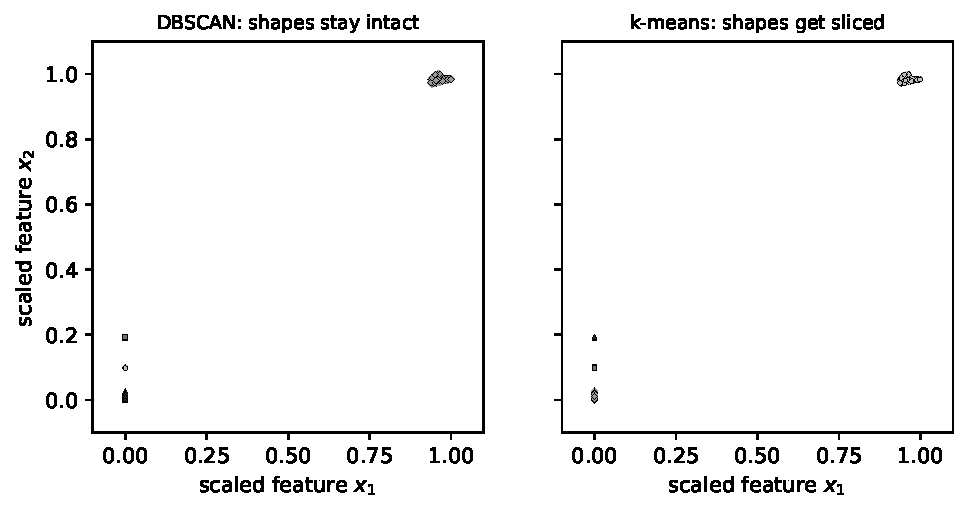
\includegraphics[width=\columnwidth]{../figures/generated/clustered_space.pdf}
\caption{Diagram B---the same points clustered two ways, one marker shape and shade per discovered class. Left: DBSCAN follows the density, so both crescents and the ring survive intact and the scattered background points are labelled noise ($-1$). Right: k-means with the correct $k=3$, which assigns every point to its nearest centre and therefore can only cut the plane into straight-edged pieces---it slices each crescent and cannot represent a ring at all. DBSCAN's labels, and nothing else, are what the KDE stage treats as ground truth.}
\label{fig:clusters}
\end{figure}

Figure~\ref{fig:surface} is the continuous decision surface, including the
$\tau=0.12$ reject plane. Figures~\ref{fig:continuous-maps} and
\ref{fig:stored-maps} compare continuous per-class density maps with the
$16\times16$ stored byte maps. The ring stays hollow in the continuous model
and remains sufficiently near zero in the table. The finest visible
approximation loss is grid resolution, not byte quantisation: the measured
worst-case quantisation error is 0.195\% of peak, within the
$1/(2\cdot255)\approx0.196\%$ bound.

\begin{figure}[!bt]
\centering
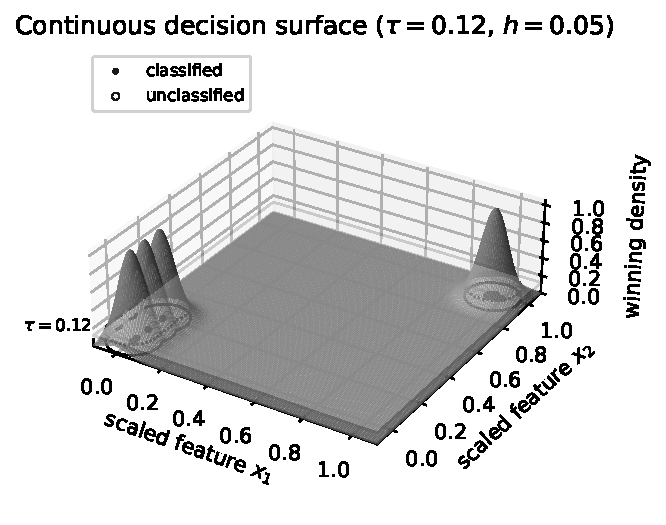
\includegraphics[width=\columnwidth]{../figures/generated/total_distribution.pdf}
\caption{Diagram C---the continuous decision surface: at every location, the largest of the three normalised class maps. This is the quantity Part 4 compares, drawn at fine resolution to show what the pipeline approximates. The surface and the flat plane at $z=\tau$ are translucent, so the training points in the feature plane below stay visible. The surface rises above $\tau$ over classified regions and dips below it over the unclassified background. The ring's hollow centre dips below $\tau$, which is why a query there is answered \textsc{unknown}. The two crescents form ridges and the ring forms a crater---shapes no centre-based method can express.}
\label{fig:surface}
\end{figure}

\begin{figure}[!bt]
\centering
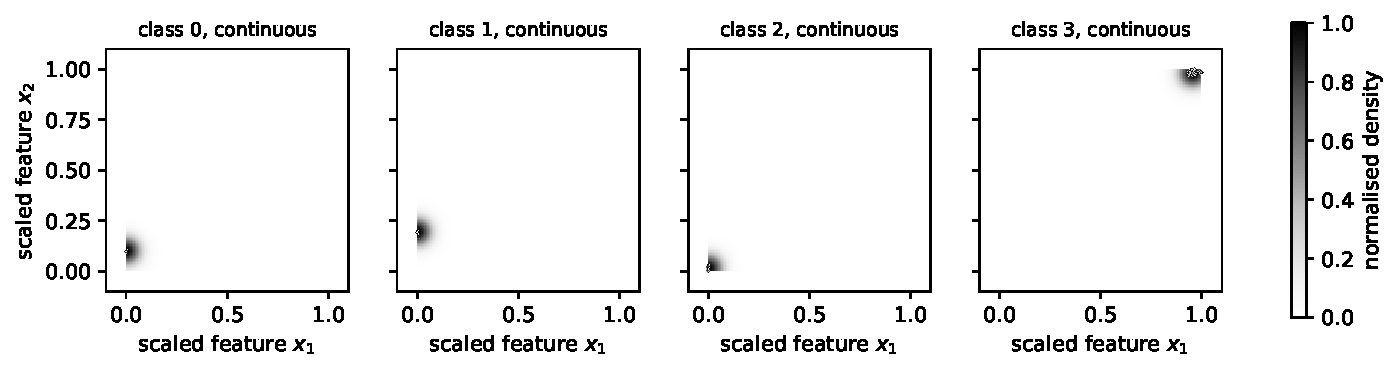
\includegraphics[width=\columnwidth]{../figures/generated/class_surfaces_continuous.pdf}
\caption{Diagram D, continuous half---each discovered class's Gaussian KDE map, normalised so its own peak is 1.0, drawn on a fine display grid. This is the continuous density as fitted, before the lookup grid coarsens it. Each class keeps its shape: two crescents and a ring whose centre stays empty.}
\label{fig:continuous-maps}
\end{figure}

\begin{figure}[!bt]
\centering
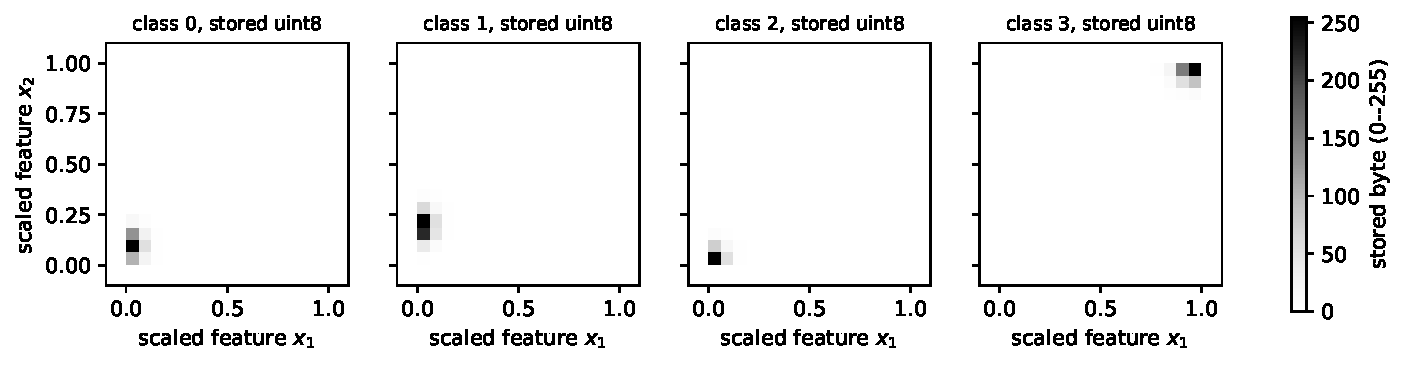
\includegraphics[width=\columnwidth]{../figures/generated/class_surfaces_discretized.pdf}
\caption{Diagram D, stored half---the same three maps as the continuous maps, now as the uint8 arrays that actually ship. Each square is one stored byte; the shade is the number. This is the complete model for these three classes: 768 bytes plus the scaling bounds, with no training points, no kernel, and no bandwidth anywhere in it.}
\label{fig:stored-maps}
\end{figure}

Table~\ref{tab:footprint} gives the memory cost of all four storage formats.
It supports shipping \texttt{uint8}: it is eight times smaller than float64
for an error below one fifth of one percent of peak. Doubling the grid to
$32\times32$ improved spatial resolution but quadrupled the uint8 tables to
3,072 bytes; the submitted $16\times16$ model is the better small-flash
trade-off.

\begin{table}[!bt]
\centering
\caption{Model footprint by storage format ($G=16$, $K=3$).}
\label{tab:footprint}
\begin{tabular}{@{}lrrr@{}}
\toprule
Storage & Bytes/cell & Per class & All classes \\
\midrule
\texttt{uint8}   & 1 & 256  & 768  \\
\texttt{uint16}  & 2 & 512  & 1536 \\
\texttt{float32} & 4 & 1024 & 3072 \\
\texttt{float64} & 8 & 2048 & 6144 \\
\bottomrule
\end{tabular}
\end{table}

With a fixed 4 kB table budget, four classes fit at $32\times32$
($4\cdot1024=4096$ bytes), while three classes fit at $36\times36$
($3\cdot1296=3888$ bytes). The latter gains resolution but leaves little
headroom and forces a class-count assumption.

Figure~\ref{fig:decision} shows an actual held-out query in row 11, column
13. Nearest lookup read bytes $(0,255,0)$ and returned distribution
$(0\%,100\%,0\%)$; bilinear read the local blend $(0,221.8,0)$ and returned
the same class and distribution. The $3\times3$ byte window for class 1 was

\[
\begin{bmatrix}
187 & 164 & 76 \\
208 & 255 & 183 \\
68 & 159 & 222
\end{bmatrix}.
\]

Of 256 cells, 127 (49.6\%) were rejected. Without the threshold, argmax
would fabricate a class throughout this unlearned region. At raw ring centre
$(4.8,1.6)$, the pipeline returned \textsc{unknown}, which is appropriate
because no class was trained there.

\begin{figure}[!bt]
\centering
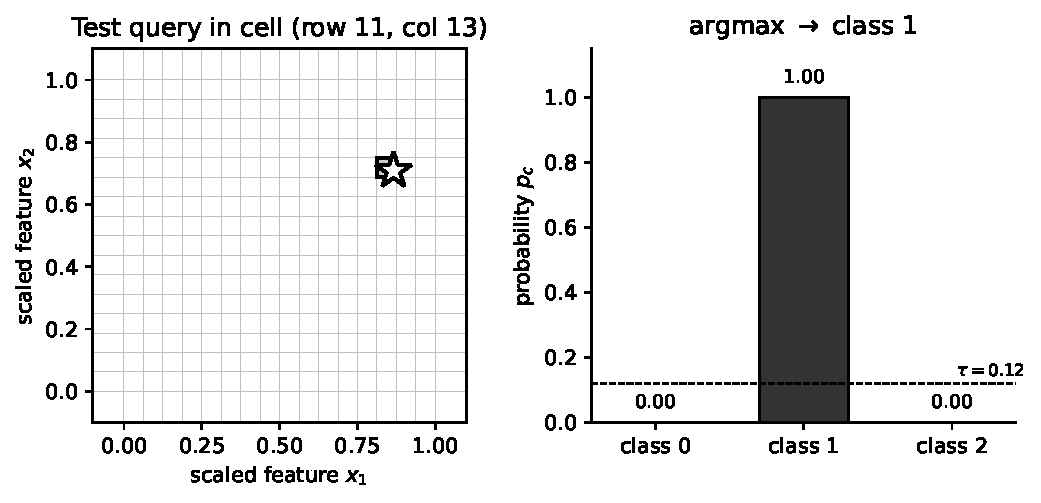
\includegraphics[width=\columnwidth]{../figures/generated/decision_map.pdf}
\caption{Diagram E---one held-out test point classified. Left: the $16\times16$ grid, with the test query and the single cell it falls in highlighted. Right: the probability read from the stored tables for each class. The decision is the tallest bar---$\arg\max_c p_c$---and the dashed line is the reject threshold $\tau$: had every bar fallen below it, the answer would be \textsc{unknown} instead.}
\label{fig:decision}
\end{figure}

On the sealed 206-point test set, stored uint8 decisions agreed with the
continuous KDE on 100.0\% of points. Table~\ref{tab:confusion} gives the
required stored-versus-continuous confusion table. Every off-diagonal value is
zero, so byte storage changed no decisions relative to the continuous artifact
on held-out data.

\begin{table}[!bt]
\centering
\caption{Stored uint8 versus continuous-KDE decisions on 206 held-out test points.}
\label{tab:confusion}
\begin{tabular}{@{}lrrrr@{}}
\toprule
Continuous / stored & c0 & c1 & c2 & unknown \\
\midrule
c0      & 69 & 0  & 0  & 0 \\
c1      & 0  & 68 & 0  & 0 \\
c2      & 0  & 0  & 63 & 0 \\
unknown & 0  & 0  & 0  & 6 \\
\bottomrule
\end{tabular}
\end{table}

\section{Limitations and remaining uncertainty}

This is evidence from one synthetic, two-dimensional dataset rather than field
data or ground-truth labels. The reported test agreement measures fidelity to
the continuous KDE's decisions, not real classification accuracy, and DBSCAN
labels could be wrong even if every plot appears plausible. The threshold was
chosen rather than derived from operating risk; a field sample outside training
bounds will be clipped into an edge cell by Algorithm~\ref{alg:lookup}, which
can yield an unwarranted label. A deployment should reject out-of-range queries
or trigger offline retraining rather than silently trust clipping.

Bandwidth sensitivity is material: low $h$ breaks maps into point-like bumps
and high $h=0.12$ smooths and fills the ring hole. Grid resolution also grows
as $G^2$, so a finer deployment must re-evaluate its flash budget and test
behaviour. Bilinear interpolation is worth its 12 reads when output controls a
gradual actuator or alarm severity near a boundary; nearest lookup is preferable
for a low-duty-cycle status indicator where fixed minimal cost matters more
than smoothing.

Two further risks remain in the offline path. DBSCAN might merge two physically
distinct operating states connected by a dense bridge, or split one real state
when its density varies; both errors would make normal-looking KDE figures
because the later stages faithfully preserve the invented labels. A change in
feature extraction or sensor calibration can invalidate the stored scaling
bounds, and a different training population can change DBSCAN labels, KDE
peaks, or selected bandwidth without changing Algorithm~\ref{alg:lookup}.
Min--max scaling still earns its place even though these two raw features have
similar ranges: it makes $\epsilon$ a fraction of the training range and makes
the device's two multiply-and-clip grid index well-defined, as
Table~\ref{tab:epsilon} demonstrates directly. Next, I would collect labelled
vibration data across machines, operating loads, and faults; validate DBSCAN
labels against maintenance records; derive $\tau$ from false-alarm and
missed-fault costs; and measure rejection and drift for data outside training
bounds.

\end{document}